\documentclass[11pt, a4paper]{article}
\usepackage[portuguese]{babel}
\usepackage[top=2cm, left=3cm, right=2cm, bottom=2cm]{geometry}
\usepackage{fontspec}
\setmainfont{Arial}
\usepackage{setspace}
\onehalfspacing
\usepackage{graphicx}
\usepackage{totpages}
\usepackage{fancyhdr}
\usepackage{url}
\usepackage[small]{caption}



\usepackage{booktabs, multirow} 
\usepackage{soul}
\usepackage[table]{xcolor}
\usepackage{changepage,threeparttable}
\usepackage{arydshln}




\pagestyle{fancy}
\fancyhead{}
\fancyfoot{}

\fancyfoot[R]{\thepage}


\usepackage{xcolor}


\begin{document}
    
    \begin{titlepage}
        \begin{center}
            
		    \textbf{PROPOSAL - FINAL UNDERGRADUATE MONOGRAPHY}
		    \vfill
		    \textbf{22/45 - HYDRAULIC CHARACTERIZATION FROM A PUMPING TEST CONDUCTED IN A COMPLEX GEOMETRY AQUIFER}
		    \vfill
		
		    \textbf{Author} \\
		    \medskip
		    Phillipe Ferreira Lima
		    \vfill
		    \textbf{Under guidance of} \\
    		\medskip
    		Prof. Ricardo Hirata \\
    		Prof. Alraune Zech
    		\vfill            
     		
\includegraphics{logo-igc.png}
     		\vfill
    		Department of Environmental and Sedimentary Geology \\
    		\medskip
    		Institute of Geosciences \\
    		University of São Paulo \\
    		2022
    		\vfill
    		
    		
        \end{center}
    \end{titlepage}
    
    %\maketitle
    
    \section{INTRODUCTION}
    \paragraph{}
    It is of great importance to have knowledge of how the hydraulics of an aquifer in which quality use will be projected, which ease and remediation of improvements to the most efficient areas. Pumping test is a commonly used technique for aquifer investigation. With this, it is possible to obtain data of the evolution of the water level drawdown curve over time and use them to characterize the hydraulic properties of the aquifer. Among the conventional methods, the most famous are Cooper-Jacob [1946] and the use of the analytical solution of Theis [1935] for the estimation of the transmissivity (T) and the calculation of the storativity (S). These conventional methods assume that the aquifers are homogeneous, that is, they have constant T and S. However, the vast majority of aquifers are heterogeneous.
    \paragraph{}
    To overcome the limitations of conventional methods in the analysis of heterogeneous aquifers, some techniques were used, such as the use of data from many observation wells during a pumping test in its stationary stage to create hydrographs and analyze the heterogeneity [Wen et al., 2010]. Methods were developed for the characterization of geostatistical hydraulic parameters of a heterogeneous aquifer, for example by using the inverse geostatistical method in Hydraulic Tomography [Yeh and Liu, 2000] and by expanding the Theis and Thiem solution for heterogeneous aquifers with log-normal distribution [Zech et al., 2012; and Zech et al., 2016]. There are several theoretical studies investigating the characterization of the heterogeneity of an aquifer using numerical models [Wu et al., 2005] and sandbox models [Berg and Illman, 2011].
    \paragraph{}
    Investigating methods for characterizing aquifer heterogeneity Wu et al. [2005] used a heterogeneous T field and Berg and Illman [2011] a sandbox with layers of different hydraulic conductivity (K). In addition, analytical methods assume that the flow of water during a pumping test is laminar and horizontal. However, there are several aquifers of complex geometry [e. g., Gutentag et al., 1984; Viguier et al., 2018] that during a pumping test they can present vertical components of water flow and can cause erroneous estimates of the T of these aquifers.
    \paragraph{} %melhorar este parágrafo
    With the hypothesis that aquifers of complex geometry can cause wrong estimates of T from the analysis of pumping test data, this project proposes to investigate possible aquifer geometries that result in a deviation between the estimated T values and the actual T values of an aquifer from the use of analytical solutions for heterogeneous aquifers since the variation of the thickness of an aquifer (complex geometry) characterizes it as a heterogeneous T aquifer. Therefore, the approach of this project will be through the use of numerical models for the creation of a field of heterogeneous thickness of aquifer of two dimensions (a horizontal and a vertical axis) that will be able to provoke water flows in the porous medium with vertical components during a pumping test. This could lead to a divergence of the estimated T values of the aquifer when compared to the actual T values from the use of analytical solutions. With this, it will be possible to measure the magnitude of the transmissivity estimation errors caused by the irregularity of the thickness of a unconfined aquifer.

    \section{OBJECTIVES}
    \paragraph{} 
    The main objective of this study is to \textbf{investigate whether aquifers with irregular geometry cause transmissivity estimation errors from the analysis of pumping test data}.
    \paragraph{}
    With the achievement of the main objective, an attempt will be made to quantify and measure the magnitude of the transmissivity estimation errors caused by the geometry of an aquifer.
    
    \section{JUSTIFICATION}
    \paragraph{}
    Aquifer heterogeneity is mostly caused by hydraulic conductivity heterogeneity and has little contribution from aquifer thickness variation. This explains the several works (Wu et al., 2005; Berg and Illman, 2011) that study the characterization of the heterogeneity of an aquifer using models with heterogeneous fields of hydraulic conductivity and transmissivity, since the second one is the integration of hydraulic conductivity. along the entire thickness of the aquifer, that is, transmissivity encompasses the concepts of hydraulic conductivity and the thickness of an aquifer. Therefore, since fluctuations in the thickness of an aquifer are almost negligible compared to its lateral continuity, the magnitude of errors in estimating hydraulic parameters in pumping tests due to vertical flows caused by the varying thickness of an aquifer will be low. However, studies to quantify this magnitude have not yet been explored and this work can be considered an innovative study.
    
    \section{PRELIMINARY BIBLIOGRAFIC} 
    
    \subsection{Pumping Test}
    \paragraph{} %pumping test
    The pumping test is a technique widely used for investigation of aquifers for many decades to characterize the hydraulic properties of an aquifer on a regional scale of hundreds of meters. This technique was originally developed with the purpose of stipulating the hydraulic potential of an aquifer for water supply. With it, it is possible to obtain data on the evolution of the water level drawdown curve over time and use them to characterize the hydraulic parameters of the aquifer. The stress caused in the pumped well will cause a drawdown of the heads in a large radial region around this well, called the cone of depression.
    \paragraph{} %estimativa de T
    Theis [1935] proposed an analytical solution that reproduces the evolution of hydraulic heads in a observation well located within the area of influence of a pumped well. With this it is possible to use this solution in an inverse method to estimate the hydraulic parameters of an aquifer, i. e. the transmissivity and the aquifer storativity. This author and other proposed analytical solutions (e.g. Hantush and Jacob, 1955; Hantush, 1960; Neuman, 1975) for the radial stress of hydraulic heads caused by a pumped well and all of this have some assumptions:
    \begin{itemize}
        \item The aquifer has constant, isotropic and homogeneous transmissivity.
        \item The aquifer is infinite in extent.
        \item The pumped well penetrates the entire thickness of the aquifer.
        \item The pumping rate in the pumped well is constant over time.
        \item The flow of water in the porous medium is laminar, horizontal and non-turbulent.
    \end{itemize}
    The estimation of the hydraulic properties of the aquifers is normally performed with the application of techniques to adjust the drawdown data observed with the theoretical curve. There are several ways to apply this technique, but the most used and famous is the Jacob Method [Cooper and Jacob, 1946], which can be applied using a paper or even with new software that uses optimization algorithms to estimate the T and S values. Meier et al. (1998) and Sanchez-Vila et al. (1999) using the Jacob method showed that the estimated parameter T is an effective transmissivity (geometric mean) of the aquifer along the entire cone of depression caused by the pumped well. These authors also showed that the transmissivity estimates using the Jacob method for a synthetic heterogeneous aquifer are very similar to the real T values. However, Wu et al. (2005) showed that the effective transmissivity estimates obtained vary over time (pumping test period) as the cone of depression increases and therefore these estimates are dependent on the size, position and degree of heterogeneity that this cone encompasses. The T values in the final stage of the pumping test (stationary stage of the cone of depression) approach the effective T values (Wu et al., 2005). These also say that the estimates of hydraulic parameters depend on the location where the data was observed (observation well) and that the hydraulic heads observed in a observation well in a heterogeneous aquifer would be a deviation from the spatial trend of the hydraulic heads predicted by the analytical solutions for a homogeneous aquifer. Therefore, using Theis' solution, which assumes that the aquifer is homogeneous, would be like comparing apples (pertubations) with oranges (trends) (Wu et al., 2005).
    \paragraph{} %aquíferos heterogêneos
    However, all aquifers present in nature violate some assumption of the conventional methods above. This is due to the fact that all aquifers have some heterogeneity and have barriers either with bodies with constant hydraulic heads (e.g. rivers and lakes) and/or limits of lateral continuity of the aquifer. Wu et al. (2005) proposed using hydrographs created from many observations wells stressed during a pumping test to obtain the hydraulic characteristics within the cone of depression in a heterogeneous aquifer.
    \paragraph{} %HT
    In order to estimate the hydraulic parameters of a heterogeneous aquifer, Hydraulic Tomography was proposed (Yeh and Liu, 2000). This technique uses an inverse geostatistical sequential method to obtain the conditioned effective hydraulic conductivity for each observation made of the hydraulic heads of a pumping test. Xiang et al. (2009) show that this technique provides hydraulic estimates of the aquifer that can predict the drawdown of hydraulic heads caused by a pumping test that was not used in hydraulic tomography analysis. However, the greater the heterogeneity of the aquifer, the greater the need for available data to characterize this aquifer. Huang et al. (2011) also show that the greater the amount of data used, the better the estimates obtained.
    \paragraph{} %ExtTheis
    Zech et al. (2012, 2016) proposed an extension of Theis and Thiem's analytical solutions to heterogeneous aquifers. With these methods the estimated hydraulic parameters are geostatistical parameters and not values for each point of the model like the previous one. Therefore, less data (observation wells) is needed to characterize the heterogeneity of an aquifer. These proposed solutions are semi-analytical solutions capable of estimating the mean ($\mu$), variance ($\sigma ^2$) and the correlation length ($\ell$) of the transmissivity in addition to being able to estimate the storativity of the aquifer. These extended solutions were obtained using the Radial Coarse Graining method to derive the effective transmissivity as a function of the aquifer statistical parameters ($\mu$, $\sigma ^2$ and $\ell$) with log-normal distribution and which depend on the radial distance ($r$) between the wells.
    \paragraph{} %análise de sensitividade
    Butler and McElwee (1990) argue that it is necessary to perform sensitivity analysis in numerical pumping test experiments. Every physical, chemical or biological system can be understood as a model with inputs that will be transformed by parameters and produce the outputs of this model. As the actual parameters are rarely known, sensitivity analysis is used in the study of how uncertainties in the input data influence the model's output data, that is, sensitivity analysis can be used to reduce the uncertainties related to the estimated parameters during a pumping test (Butler and McElwee, 1990). The most used ways to calculate sensitivity are: perturbation, analytical, direct method, and the adjoint method. Kabala (2001) says that the sensitivity of the drawdown of the hydraulic heads of a well during a pumping test increases rapidly with time until the water flow in the walls of the tubular well equals the pumping rate. After a plateau it starts to decrease slowly with time. On the other hand, the sensitivity of T decreases during the storage phase and after this stage it converges to a single value. However, currently there are software and codes that perform the sensitivity calibration in a computerized and automatic way through the use of optimizing algorithms.
    
    \subsection{Numerical Model}
    \paragraph{} %teste de bombeamento em modelo numérico
    Computer numerical models are increasingly applied as a way of experimenting with natural phenomena. This is due to the advancement of computational processing capacity and the advancement of software that allow the use of numerical models in the simulation of more complex phenomena in a easier way. These simulations applied to the analysis of pumping tests have been in use for at least 40 years (e.g. Rushton and Booth, 1976; Lakshminarayana and Rajagopalan, 1978; Rathod and Rushton, 1991; Rutledge, 1991). The main utility of conducting pumping tests on numerical models is that the premises and properties to be calibrated can be chosen by the user and that during the model calibration process it is possible to obtain an insight into the water flow in the conceptual model of the aquifer and the uncertainties of its analysis (Johnson et al., 2001).
    \paragraph{} %MODFLOW
    Several software were and are being developed with pre-configured codes of finite differences and finite elements in order to facilitate the construction of models and allowing the user to focus on the analysis of the experiment. An example is the MODFLOW (Harbaugh and McDonald, 1996) in which it is possible to build models of one, two or three dimensions to conduct pumping tests and which brought the user's ability to use cylindrical coordinates to analyze the drawdown of the hydraulic head during a pumping test (Reily and Harbaugh, 1993).
    \paragraph{} %modelo numérico livre de noise
    The use of numerical modeling as a laboratory for conducting experiments is widely used since this method can isolate what really matters in the study of a process. Thus, experiments performed using numerical models of aquifers and the execution of pumping tests make the results noise-free. These noises can be characterized as errors in measurements that may originate in the process of collecting hydraulic heads from observation wells and/or measuring the flow of pumped well. Another type of phenomenon that can generate noise in the data is the variation in the pumping rate due to technical difficulties during the process. There are still several other types of noise that can impact the data produced during a pumping test, e.g. Noordbergum effect, leakage, barometric effects, and others.
    \paragraph{} %principio da reciprocidade
    Numerical pumping test models, in addition to being free from noise that can cause errors, have the principle of reciprocity. This principle was initially applied in the field of electromagnetic fields proposed by Lorentz and says that the stress applied at point A and the effect measured at point B will have the same effect at point A for the same stress applied at point B in processes that occur in heterogeneous environments. For the pumping test case this principle was analyzed by Bruggeman [1972] for the steady and transient flow of groundwater in heterogeneous media and translates for this area as the following: the drawdown curve in the well A caused by the pumping the well B it will be the same drawdown curve seen in well B caused by pumping well A. Delay et al. [2011] further says that the principle of reciprocity in pumping test is guaranteed between a pumping well and a observation well during a pumping test with more than one observation wells regardless of the initial pre-pumping conditions for darcyan flows in heterogeneous medium. The infraction of this principle can be a consequence of physical factors such as cracks between points A and B, errors originated in data collection and infringement of the assumptions of the governing equations, such as turbulent water flow, vertical water flux, etc.
    
    \section{MATERIALS AND METHODS}
    \paragraph{} %resumo - intro
    All stages of the algorithm, that is, the numerical model, simulation of the pumping test, characterization of the hydraulic parameters, as well as the subsequent variation of the aquifer geometry will be implemented in Python. Python packages that are part of the GeoStat-Framework will be used ( \url{https://geostat-framework.org} ), such as ogs5py, welltestpy and anaflow.
    \paragraph{} %modelo numérico 
    The numerical model will be created using the Python library ogs5py and will simulate an aquifer where the pumping test will be performed. The ogs5py library is a Python API of the OpenGeoSys5 (OGS5) scientific modeling software. OpenGeoSys uses numerical methods to simulate thermal, hydraulic, mechanical, and chemical processes in porous or fractured media. OGS5 uses finite element method to solve partial differential equations governing subsurface flow and transport processes [Müller et al., 2020].
    \paragraph{} %teste de bombeamento
    The pumping test is performed by pumping groundwater through a well and measuring the water flow and the drawdown of the water level in the pumped well. During the execution of this technique the well is pumped for several hours and can last for weeks. This will cause a drawdown of the hydraulic heads at a radial distance around the pumped well, characterizing the cone of depression caused by the pumping test. The measurements of the hydraulic heads in the observation wells can be made by piezometers located in these wells, far from the well that will be pumped the water. These measurements can be applied to a vertical flow equation of water in a well to estimate the hydraulic characteristics of the pumped aquifer [Kruseman and De Ridder, 2000]. Before carrying out this type of test, it is necessary to collect information such as subsurface geological characteristics, aquifer type, aquifer thickness and lateral continuity, etc. [Kruseman and De Ridder, 2000].
    \paragraph{} %inferência de T
    The estimation of the aquifer transmissivity will be obtained through the analysis of the data resulting from the pumping tests in the numerical model using the Welltestpy library. Welltestpy is a Python library that provides tools for inferring hydraulic parameters of aquifers from pumping test data. Among the estimators present in this package, solutions that take into account the heterogeneity of the aquifer such as ExtTheis [Zech et al., 2016] will be used, since the variation in the thickness of an aquifer characterizes it as having heterogeneous T.
    \paragraph{} %ExtTheis
    The extended Theis solution is an expanded Theis solution used to inversely infer geostatistical parameters from transient pumping test data in heterogeneous T-field aquifers using the Radial Coarse Graining method [Zech et al., 2016]. An example of successful use of this library and this solution is presented in Müller et al [2021]. This semi-analytical solution will be used with the help of the welltestpy library. This library provides tools to infer hydraulic parameters from pumping test data in heterogeneous aquifers. Any pump test campaign can be configured in the package with a few lines of Python code and from there use this data to estimate the hydraulic parameters of the aquifer (Fig. \ref{fig:welltestpy}). In addition, this package provides tools that assist in various data processing. \\
    
    \begin{figure}[h]
        \centering
        \captionsetup{justification=centering}
        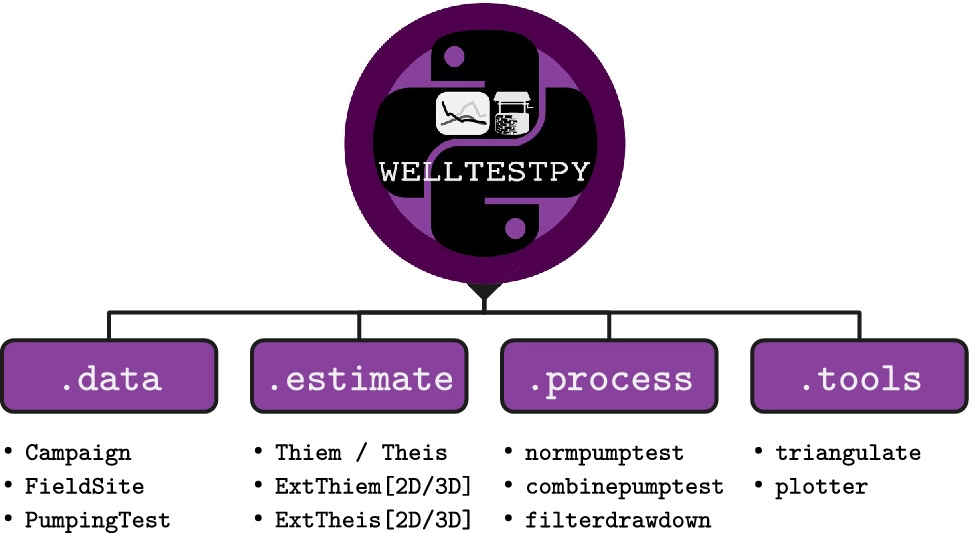
\includegraphics[height=2.5in]{welltestpy.png}
        \caption{Organization chart of the welltestpy package for the Python language with its sub-packages and main features.}
        \label{fig:welltestpy}
    \end{figure}
    
    \paragraph{} %algoritmo MCMC
    The variation of the aquifer geometry will be implemented in the algorithm using the central idea of the Reversible Jump Markov Chain Monte Carlo algorithm [Green, 1995]. This algorithm, which is also called birth death Markov Chain Monte Carlo, extends the use of the Metropolis-Hastings algorithm where the proposed distribution not only moves the points within the model space, it also moves between the states of the model space, that is, the number of dimensions of the model varies [Green, 1995]. However, this project will initially only use the idea of dimensionality change in a Monte Carlo simulation and will not use the Bayesian approach to approach a specific distribution or an expected value.
    \paragraph{} %análise dos dados 
    The analysis of the transmissivity values obtained will be done using the anaflow library. It provides various analytical and semi-analytical solutions for water flow in porous media during a pumping test. The transmissivity values inferred using the estimators from the welltestpy library will be used to plot a curve of drawdowns as a function of the radial distance of the pumped well and compared with the observations of these drawdowns made by the model. Another example of analysis to be performed will be to compare the predicted drawdown using the estimated parameters with the observed drawdown of the numerical model (Fig. \ref{fig:huang}). With this it will be possible to measure graphically how good are the estimates of the hydraulic parameters obtained.
    
    \begin{figure}[h]
        \centering
        \captionsetup{justification=centering}
        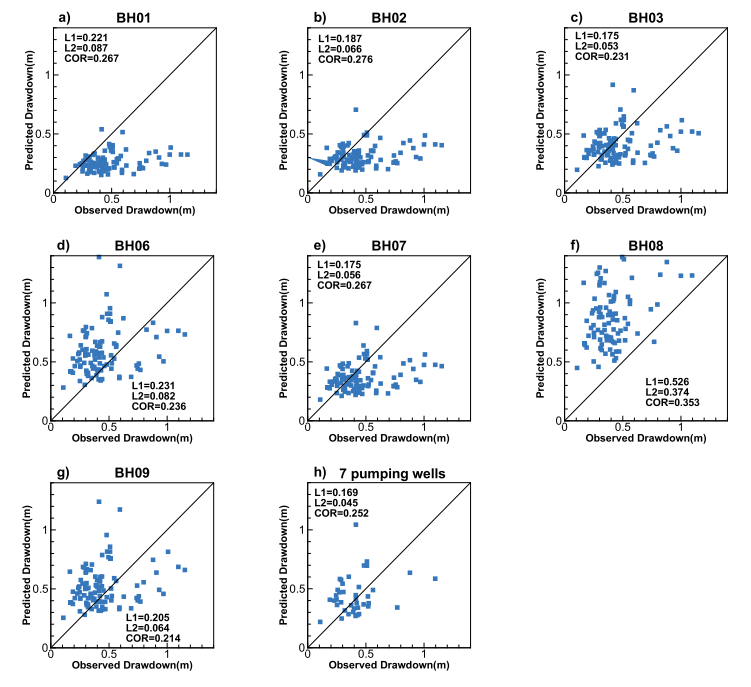
\includegraphics[height=5.5in]{huang-et-al.png}
        \caption{Example of data analysis using scatter plots of observed drawdown versus predicted drawdown for various observations wells. Fonte: Huang et al., 2011}
        \label{fig:huang}
    \end{figure}
    
    
    \section{EXPECTED DEVELOPMENT} \label{sec:desen}
    \paragraph{} %resumo do que será feito - parte 1
    The hypothesis will be tested with the creation of a numerical model of an aquifer with a non-constant thickness. Therefore, instead of creating a T field or a K field, in this project what will be directly responsible for promoting the heterogeneous character to the aquifer will be a heterogeneous field of the thickness of this aquifer. Only with this will it be possible to generate vertical flow components to later be able to measure the magnitude of the deviations of the estimated t values in relation to the expected T values. With this model, pumping tests will be conducted and data collected. These data will serve as a source for estimating the transmissivity of the aquifer through the use of analytical solutions that consider heterogeneity in the aquifers.
    \paragraph{} %resumo - parte 2
    The above procedures will be part of an iteration of the Monte Carlo algorithm. For each new iteration the thickness of the aquifer model will vary and then a new transmissivity estimate will be performed with the data obtained with the new pumping test conducted. This will make the algorithm, throughout the simulation, estimate T for several aquifers with different geometries. Thus, at the end of the Monte Carlo simulation, the results will be the depth values that form the aquifer model, the estimate of T and the real value of T for each iteration. From this, it will be possible to identify for which geometry there was a greater deviation from the expected T value compared to the real T value of the aquifer model. It is important to highlight that this algorithm will have restrictive conditions so that during the iterations the pumping tests will be conducted only in aquifer geometries that are plausible in nature.
    \paragraph{} %etapas da elaboração do projeto
    The project will be carried out in stages and the algorithm will be developed gradually, starting with simpler models and adding complexity as the tests present positive feedback. The objective of this approach is to avoid complex errors that can become difficult to solve within the duration of the project and to always have results so that at the end of the project, even if possibly incomplete due to some unforeseen event, there is analysis and discussion of the results. With this in mind, the expected development of this project will take place with the following steps:
        \begin{enumerate}
            \item Creation of a 2D numerical model of a homogeneous aquifer with constant thickness and conduction of the pumping test.
            \item Improve the previous model by making the thickness vary along the horizontal axis and conducting the pumping test. Tests with different observation well and pumping well positions and for different aquifer thicknesses (vertical axis).
            \item Start the production of the Markov Chain Monte Carlo algorithm in which each iteration will only be responsible for varying the aquifer thickness without carrying out the pumping test. This geometry variation will occur at each iteration at the interface between the aquifer and an impermeable bedrock so that it will have four possibilities of change chosen at random. Since the geometry of the aquifer will be defined by nodes these changes will change the values of these nodes and the four possibilities are:
            \begin{itemize}
                \item increase the depth of a random node
                \item decrease the depth of a random node
                \item create a new node with random position
                \item delete any node
            \end{itemize}
            \item Add the pumping test to the previous stage and collect the data for each iteration. Only one observation well and one pumping well will be used for pumping.
            \item Add the code responsible for estimating the transmissivity for each iteration using the data generated by the pumping tests and storing the estimated values of T with the parameters that will produce it (e.g. node positions, observation wells and pumping well positions and the model's actual T value).
            \item Add restrictions to the algorithm so that the variation of node depths does not exceed a certain value, taking into account the difference in depths with neighboring nodes and the distances between them. This will ensure that there are no iterations with aquifer geometries that are not plausible to find in nature.
            \item Improve the algorithm to separate the data from the iterations that showed the greatest deviation from the estimate of T values and the expected (actual) T values.
            \item Add more monitoring wells to the algorithm.
        \end{enumerate}
    \paragraph{} %análise e interpretação dos resultados a cada etapa
    After the success of each of the steps, the aquifer transmissivity will be estimated, based on the data produced by the pumping tests, using analytical solutions that assume a heterogeneous aquifer (with the exception of the first step, which will use the Theis solution) . The estimates that most deviate from the expected values will be analyzed using analytical solutions comparing the observed drawdown from the pumping test with the drawdown curve predicted by analytical solutions using the estimates obtained. The different estimate values for each observation well will still be interpreted according to what the bibliography says. As well as the identification of possible patterns of aquifer geometry that cause greater deviation from the expected T values and correlate it with geological/tectonic environments that can promote such geometries. Finally, a research will be carried out on the possible factors that may cause estimation errors and compare their magnitude with the magnitude of the errors found in this project in order to keep in mind the importance influence of geometry in the estimates of transmissivity in heterogeneous aquifers from pumping tests. .
    
    \section{ACTIVITIES SCHEDULE} %fazer tabela com layout bonito
    \paragraph{}
    The activities to perform this work is presented in the table \ref{tab:cronograma}. The creation of the initial model corresponds to steps 1 and 2 of the section \ref{sec:desen}, while the elaboration of the algorithm corresponds to the other steps.
    
    \begin{adjustwidth}{-2.5 cm}{-2.5 cm}\centering
    \begin{threeparttable}[!htb]
        \caption{Schedule of activities to be carried out.}\label{tab:cronograma}
        \scriptsize
        \begin{tabular}{|lr|r|r|r|r|r|r|r|r|r|}\hline%\toprule
            \textbf{Activity} &\textbf{Month} &May &Jun &Jul &Aug &Sep &Out &Nov &Dec \\\hline%\midrule
            Bibliographic Research & &\cellcolor[HTML]{6aa84f} &\cellcolor[HTML]{6aa84f} &\cellcolor[HTML]{6aa84f} &\cellcolor[HTML]{6aa84f} &\cellcolor[HTML]{6aa84f} &\cellcolor[HTML]{6aa84f} &\cellcolor[HTML]{6aa84f} & \\ \hline
            Initial Model Development & &\cellcolor[HTML]{6aa84f} &\cellcolor[HTML]{6aa84f} & & & & & & \\ \hline
            Algorithm Development & & &\cellcolor[HTML]{6aa84f} &\cellcolor[HTML]{6aa84f} &\cellcolor[HTML]{6aa84f} &\cellcolor[HTML]{6aa84f} &\cellcolor[HTML]{6aa84f} & & \\ \hline
            Analysis of Preliminary Results & & &\cellcolor[HTML]{6aa84f} &\cellcolor[HTML]{6aa84f} &\cellcolor[HTML]{6aa84f} &\cellcolor[HTML]{6aa84f} &\cellcolor[HTML]{6aa84f} & & \\ \hline
            Preparation of the Partial Report & & & &\cellcolor[HTML]{6aa84f} &\cellcolor[HTML]{6aa84f} & & & & \\ \hline
            Analysis of Final Results & & & & & & & &\cellcolor[HTML]{6aa84f} & \\ \hline
            Preparation of the Final Monograph & & & & & & &\cellcolor[HTML]{6aa84f} &\cellcolor[HTML]{6aa84f} & \\ \hline
            Preparation of the Defend Presentation & & & & & & & & &\cellcolor[HTML]{6aa84f} \\ 
            \hline%\bottomrule
        \end{tabular}
        \end{threeparttable}
    \end{adjustwidth}
    
    
    \section{EXECUTION FEASIBILITY}
    \paragraph{}
    The project data will be generated computationally as well as the analysis of the results. In this way, logistical and financial conditions will not be a problem for the feasibility of executing the project. For the instrumental conditions, the personal computer of the author of this work will be used. Since the proposed model requires computational processing power beyond that available on the author's personal computer, the use of a supercomputer located at the Institute of Astronomy and Geophysics of the University of São Paulo will be required to execute the algorithm.
    
    \section{REFERENCES} 
    
    \paragraph{}
    Berg, S. J., and W. A. Illman, 2011. Capturing aquifer heterogeneity: Comparison of approaches through controlled sandbox experiments, Water Resour. Res., 47, W09514, \\doi:10.1029/2011WR010429.
    
    
    Bruggeman, G. A. (1972), The reciprocity principle in flow through heterogeneous porous media, in Development in Soil Science, Fundamental of Transport Phenomena in Porous Media, vol. 71, pp. 136–149, IAHR, Elsevier, Amsterdam.
    
    
    Butler, J.J. Jr., and C.D. McElwee. 1990. Variable-rate pumping tests for radially symmetric nonuniform aquifers. Water Resources Research 26, no. 2: 291-306.

    
    Cooper, H. H., Jr., and C. E. Jacob, 1946. A generalized graphical method for evaluating formation constants and summarizing well-field history, Eos Trans. AGU, 27(4), 526–534.
    
    
    Delay, F., P. Ackerer, and A. Guadagnini (2011), Theoretical analysis and field evidence of reciprocity gaps during interference pumping tests, Adv. Water Resour., 34(5), 592–606.
    
    
    Green, P.J., 1995. Reversible jump Markov chain Monte Carlo computation and Bayesian model determination, Biometrika, 82, 711–32.
    
    
    Gutentag, E. G., F. J. Heimes, N. C. Krothe, R. R. Luckey, and J. B. Weeks. 1984. Geohydrology of the High Plains Aquifer in parts of Colorado, Kansas, Nebraska, New Mexico, Oklahoma, South Dakota, Texas, and Wyoming. U.S. Geological Survey Professional Paper 1400-B.
    
    
    Hantush, M. S. and C. E. Jacob. 1955. Nonsteady radial flow in an infinite leaky aquifer. Transactions of the American Geophysical Union, 36, 95–100.


    Hantush, M. S. 1960. Modification of the theory of leaky aquifers. Journal of Geophysical Research, 65, 3713–3725.

    
    Harbaugh, A.W., and McDonald, M.G., 1996. User’s documentation for MODFLOW-96, an update to the U.S. Geological Survey modular finite-difference ground-water flow model: U.S. Geological Survey Open-File Report 96–485, 56 p.
    
    
    Huang S.-Y., Wen, J. -C, Yeh, T.-C. J., Lu, W., Juan, H.-L., Tseng, C.-M., Lee, J.-H., Chang, K.-C., 2011. Robustness of joint interpretation of sequential pumping tests: Numerical and field experiments, WATER RESOURCES RESEARCH, VOL. 47, W10530, \\doi:10.1029/2011WR010698
    
    Johnson, G. S., Cosgrove, D. M., Frederick, D. B., 2001. A Numerical Model and Spreadsheet Interface for Pumping Test Analysis, GROUNDWATER 39, No. 4, 582–592.

    
    Kabala, Z. J., 2001. Sensitivity analysis of a pumping test on a well with wellbore storage and skin, Advances in Water Resources, Volume 24, Issue 5, Pages 483-504, ISSN 0309-1708, https://doi.org/10.1016/S0309-1708(00)00051-8.

    
    Kruseman, G. P., N. A. de Ridder. 2000. Analysis and Evaluation of Pumping Test Data. Second Edition, International Institute for Land Reclamation and Improvement.
    
    
    Lakshminarayana, V., and S.P. Rajagopalan. 1978. Digital model studies of steady-state radial flow to partially penetrating wells in unconfined anisotropic aquifers. Journal of Hydrology 38, 249-262.

    
    Müller, S., A. Zech, F. Heße. 2020. ogs5py: A Python-API for the OpenGeosys 5 Scientific Modeling Package. Groundwater, 59, pp. 117-122, https://doi.org/10.1111/gwat.13017
    
    
    Müller, S., C. Leven, P. Dietrich, S. Attinger, A. Zech. 2021. How to Find Aquifer Statistics Utilizing Pumping Tests Studies Using welltestpy. Groundwater, 60, pp. 137-144, \\https://doi.org/10.1111/gwat.13121
    
    
    Neuman, S. P. 1975. Analysis of pumping test data from anisotropic unconfined aquifers considering delayed gravity response. Water Resources Research, 11, 329–342.
    
    
    Rathod, K.S., and K.R. Rushton. 1991. Interpretation of pumping from two zone layered aquifers using a numerical model. Ground Water 29, no. 4: 499-509. 

    
    Reilly, T.E., and A. W. Harbaugh. 1993. Simulation of cylindrical flow to a well using the U.S. Geological Survey Modular Finite-Difference Ground-Water Flow Model. Ground Water 31, no. 3: 489-494.

    
    Rushton, K.R., and S.J. Booth. 1976. Pumping-test analysis using a discrete time-discrete space numerical model. Journal of Hydrology 28, 13-27.

    
    Rutledge, A.T. 1991. An axisymmetric finite-difference flow model to simulate drawdown in and around a pumped well. USGS Water Resources Investigations Report 90-4098.
    
    
    Theis, C. V. (1935), The relation between lowering the piezometric surface and the rate and duration of discharge of a well using ground water storage, Eos Trans. AGU, 16, 519–524.
    
    
    Wen, J. C., C. M. Wu, T.-C. J. Yeh, and C. M. Tseng (2010), Estimation of effective aquifer hydraulic properties from an aquifer test with muti-well observations (Taiwan), Hydrogeol. J., 18, 1143–1155, doi:10.1007/ s10040-010-0577-1
    
    
    Wu, C. M., T.-C. J. Yeh, J. Zhu, T. H. Lee, N. S. Hsu, C. H. Chen, and A. F. Sancho (2005), Traditional analysis of aquifer tests: Comparing apples to oranges?, Water Resour. Res., 41, W09402, doi:10.1029/2004WR003717.
    
    
    Xiang, J., T.-C. J. Yeh, C.-H. Lee, K.-C. Hsu, and J.-C. Wen (2009), A simultaneous successive linear estimator and a guide for hydraulic tomography analysis, Water Resour. Res., 45, W02432, doi:10.1029/2008WR007180.

    
    Zech, A., S. Muller, J. Mai, F. Heße, and S. Attinger. 2016. `Extending Theis' solution: Using transient pumping tests to estimate parameters of aquifer heterogeneity. Water Resources Research 52, no. 8: 6156–6170. https://doi.org/ 10.1002/2015WR018509
    
    
    Zech, A., C.L. Schneider, and S. Attinger. 2012. The extended Thiem’s solution Including the impact of heterogeneity. Water Resources Research 48, no. 10: W10535. https://doi .org/10.1029/2012WR011852
    
    
\end{document}

